\documentclass[notitlepage,letterpaper,pdftex,12pt,final]{article}
%\documentclass[notitlepage,letterpaper,pdftex,12pt,draft]{article}
% article < report < book ; preable material follows
%
% This file is mostly boilerplate that you can copy and tweak.
% The true material is in included files.  ../common should hold
% things that more than one document might need.  The Makefiles
% should likewise be mostly boilerplate with minor tweaks.
%

% (un)comment to (see)hide full paths to files actually used
% however, you'll need to override the TEXOPT= setting to batchmode
% made in the Makefile.
\listfiles

\addtolength\textwidth{1.7in}
\addtolength\oddsidemargin{-0.95in}
\addtolength\evensidemargin{-0.95in}
\addtolength\marginparwidth{-0.95in}
\typeout{textwidth is \the\textwidth}

% useful to block out portions of text
\usepackage{ifthen}
% to allow defining our own colors
\usepackage[dvipsnames]{xcolor}
% makes hyperlinks work
\usepackage{hyperref}
\hypersetup{colorlinks=true,linkcolor=darkblue,citecolor=darkgreen}
% for figures; insert [draft] before {...} not to see imgs
\usepackage{graphicx}
% for small figures surrounded by text
\usepackage{wrapfig}
% for control over headers and footers
\usepackage{fancyhdr}
\pagestyle{fancy}
\fancyhf{}
% for handling acronyms
\usepackage[printonlyused]{acronym}

% for bibliographies if needed
\usepackage[utf8]{inputenc}
\usepackage[english]{babel}
\usepackage[backend=biber,style=numeric,sorting=none]{biblatex}
%\usepackage[backend=bibtex,style=numeric,sorting=none]{biblatex}
\addbibresource{hops.bib}
% context-sensitive quotes
\usepackage{csquotes}
% underline for emphasis: \uline etc
\usepackage{ulem}
% for generating outlines
\usepackage{outlines}
\usepackage{enumitem}

% for bold math
\usepackage{bm}
% for serious math which we may have in a few places (eventually)
\usepackage{amsmath}
% equations include section number
\numberwithin{equation}{section}

% for marginal notations concerning geodesy
\usepackage{marginnote}

% to go back to default after \ragged commmands
\usepackage{ragged2e}

% see common/shortcuts.tex for what is defined in this file
%
% a file of commands to save typing
%

% commonly used things
\newcommand{\eg}{\textit{e.g.}}
\newcommand{\EG}{\textit{E.g.}}
\newcommand{\ie}{\textit{i.e.}}
\newcommand{\IE}{\textit{I.e.}}
\newcommand{\etc}{\textit{\&c.}}
\newcommand{\Sec}{Section}
\newcommand{\Fig}{Figure}
\newcommand{\Tab}{Table}
\newcommand{\App}{Appendix}

% for a work in progress:
\newcommand{\FIX}[1][fixme]{{\color{red}#1}}
\newcommand{\TBC}{{\color{red}TBC}}
\newcommand{\TBD}{{\color{red}TBD}}
\newcommand{\TBR}{{\color{red}TBR}}
\newcommand{\FIXME}[1][]{{\color{red}FIXME -- #1}}

% specific to this project
\newcommand{\MHO}{MIT-HOPS}
\newcommand{\HOPS}{HOPS}

% standard colors
\definecolor{darkblue}{rgb}{0,0,.5}
\definecolor{darkgreen}{rgb}{0,.5,0}
\definecolor{darkred}{rgb}{.5,0,0}
\definecolor{violet}{rgb}{.4,0.,.7}

% for coping with geodetic things
\newboolean{geos}
\setboolean{geos}{true}% or false to hide geodetic marginal notations
%
\definecolor{boxfrcolor}{rgb}{.50,.20,.00}
\definecolor{boxbgcolor}{rgb}{0.9,.98,.98}
\definecolor{boxfgcolor}{rgb}{0.4,0.0,0.0}
% \geomargin{footnote comment}
% \geomargin[{\color{..}box note}]{footnote comment}
\newcommand{\geobox}[1]%
{{\parbox{10mm}{\small\textit{\fcolorbox{boxfrcolor}{boxbgcolor}{#1}}}}}
\newcommand{\geomargin}[2][{\color{boxfgcolor}geodesy}]%
{\ifthenelse{\boolean{geos}}{% if:
\marginnote{\protect\geobox{#1}}\footnote{#2}}{% else: show nothing
}}

% for itemizing requirements
\newcounter{req}
\newcommand{\reqid}[1]{\item[\refstepcounter{req}#1-\thereq]}

%
% eof
%

\setboolean{geos}{true}% or false to hide geodetic marginal notations

% control options
\newboolean{skipappendix}
\setboolean{skipappendix}{false}

% at some point this gets frozen
\newcommand{\recdate}{\today}

\makeatletter
\newcommand\urlfootnote@[1]{\footnote{\url@{#1}}}
\DeclareRobustCommand{\urlfootnote}{\hyper@normalise\urlfootnote@}
\makeatother

\usepackage{adjustbox}

\usepackage[font=small]{caption}
\usepackage{xspace}
\usepackage{float}


\usepackage{graphicx}
\usepackage{amsmath}
\usepackage{amsfonts}
\usepackage{amssymb}
\usepackage{multirow}
\usepackage{subcaption}
% \usepackage{lineno}
\usepackage{listings}
\usepackage{microtype}
\usepackage{placeins}
%\usepackage[x11names]{xcolor}
\usepackage{footnote}
\usepackage{adjustbox}

\usepackage[T1]{fontenc}
\usepackage[scaled]{beramono}
\newcommand\Small{\fontsize{9}{9.2}\selectfont}
\newcommand\Normal{\fontsize{12}{12.3}\selectfont}
\newcommand*\LSTfont{\Small\ttfamily\SetTracking{encoding=*}{-60}\lsstyle}
\newcommand*\LSTfontNormal{\Normal\ttfamily\SetTracking{encoding=*}{-60}\lsstyle}

\usepackage{listings}


\lstset{ %
  backgroundcolor=\color{white},   % choose the background color; you must add \usepackage{color} or \usepackage{xcolor}
  basicstyle=\LSTfont,        % the size of the fonts that are used for the code
  breakatwhitespace=false,         % sets if automatic breaks should only happen at whitespace
  breaklines=true,                 % sets automatic line breaking
  captionpos=b,                    % sets the caption-position to bottom
  commentstyle=\color{gray},    % comment style
  deletekeywords={...},            % if you want to delete keywords from the given language
  escapeinside={\%*}{*)},          % if you want to add LaTeX within your code
  extendedchars=true,              % lets you use non-ASCII characters; for 8-bits encodings only, does not work with UTF-8
  frameshape={RYR}{Y}{Y}{RYR},	                   % adds a frame around the code
  keepspaces=true,                 % keeps spaces in text, useful for keeping indentation of code (possibly needs columns=flexible)
  keywordstyle=\color{blue},       % keyword style
  language=C++,                 % the language of the code
  otherkeywords={*,...},           % if you want to add more keywords to the set
  numbers=none,                    % where to put the line-numbers; possible values are (none, left, right)
  numbersep=5pt,                   % how far the line-numbers are from the code
  numberstyle=\tiny\color{gray}, % the style that is used for the line-numbers
  rulecolor=\color{black},         % if not set, the frame-color may be changed on line-breaks within not-black text (e.g. comments (green here))
  showspaces=false,                % show spaces everywhere adding particular underscores; it overrides 'showstringspaces'
  showstringspaces=false,          % underline spaces within strings only
  showtabs=false,                  % show tabs within strings adding particular underscores
  stepnumber=2,                    % the step between two line-numbers. If it's 1, each line will be numbered
  stringstyle=\color{red},     % string literal style
  tabsize=2,	                   % sets default tabsize to 2 spaces
  title=\lstname                   % show the filename of files included with \lstinputlisting; also try caption instead of title
}


\usepackage{algorithm}
\usepackage{algpseudocode}
\renewcommand{\algorithmicrequire}{\textbf{Input:}}
\renewcommand{\algorithmicensure}{\textbf{Output:}}

\usepackage{tabularx}
\newcolumntype{L}{>{\raggedright\arraybackslash}X}


%\usepackage{tikz}
%\usepackage{pgfplots}
%\usetikzlibrary{positioning}
%\usetikzlibrary{shapes.geometric, arrows}
%\pgfplotsset{compat=1.11}
\usepackage[margin=0.9in]{geometry}

\newcommand\tikzmark[2]{%
  \tikz[remember picture,overlay]\node[arrow,draw] (#1) {#2};}


%\usepackage[printwatermark]{xwatermark}
%\newwatermark[pages=2-30,color=gray!25,angle=45,scale=5,xpos=0,ypos=0]{DRAFT}


%\usepackage{etoolbox}
%\makeatletter
%\patchcmd{\@verbatim}
%  {\verbatim@font}
%  {\verbatim@font\tiny}
%  {}{}
%\makeatother

%\usepackage{ifthen}

%\let\endtitlepage\relax


\begin{document}
\DeclareGraphicsExtensions{.png, .jpg, .pdf}
% best to put figures in subdirs
%\graphicspath{{figs/}{scans/}}

% for subsequent pages
\setlength\headheight{15pt}
\fancyhead[L]{HOPS}
\fancyhead[C]{}
\fancyhead[R]{Specifications}
\fancyfoot[R]{Page \thepage\ of\ \pageref{page:LastPage}}
\fancyfoot[L]{\recdate}

\title{ngEHT Specifications for a new HOPS}

\author{%
\LARGE John Barrett, Geoff Crew, Dan Hoak and Violet Pfeiffer \\
\Large MIT Haystack Observatory}
\date{Version 1.0, \recdate}
\maketitle
\normalsize

\renewcommand\abstractname{Executive Summary}
\abstract{%
\large
This document lays out the general architecture adopted for
this rewrite of \ac{HOPS}.  The orginal version of \ac{HOPS}
was written with a mix of C and F77 with some dependencies
that are becoming a challenge to satisfy.  The new architecture
will involve a mix of C/C++ for the lower-layers, and add a
Python layer to better support human interactions.  The new
implementation will be more modular, and easier to support
for the coming decades.
}

%   * Architecture definition
%   * Language selection
%   * Build system selection
%   * Parallel support definition
%   * Interactivity definition
%   * External package identification
%   * New objects specification
%   * New library specification
%   * New program specification





% \begingroup . . . \endgroup can be used to keep things together
% and/or an explicit page break and/or adjust spacing as needed so
% it looks presentable.  Uncomment the sections you need.
%\begingroup
%\renewcommand\contentsname{Contents}
%\renewcommand\listfigurename{Figures}
%\renewcommand\listtablename{Tables}
%\vspace{24pt}\hrule
\pagebreak
\tableofcontents
%\vspace{24pt}\hrule
%\pagebreak
%\listoffigures
%\vspace{24pt}\hrule
%\listoftables
%\vspace{24pt}\hrule
%\endgroup

% it is sometimes cleaner to start sections on new pages in a longer
% document--then changes to each section don't repage everything.
\pagebreak

\section{Introduction}

This document is intended to record the design decisions made in specifying how the HOPS re-development project undertakes the
re-design and re-implementation of the VLBI post-processing software HOPS. As this is a software project there is a certain
degree of ongoing flexibility that is needed in order to obtain an optimal result upon completion. Therefore, this 
draft document will be updated periodically along with the software as it is built out. The initial focus will be to determine
the of components of the design and their dependencies which must be in place as basic infrastructure before further development
can take place.



% break document into appropriate portions
%\input{tbd}

%\pagebreak
%\input{specs-intro}

\pagebreak

\section{General Architecture}
\label{sec:architecture}


The goal of the re-developed HOPS architecture is provide a component-based design which allows for a greater degree of flexibility
in the types of operations that may be applied to VLBI data during fringe fitting, and avoid the semi-monolithic approach used in the past.
To do this, the software package to be delivered will primarily comprise of a set of loosely coupled libraries which can be composed
into an variety of calibration and fringe-fitting applications. Moreover, rather than attempting to identify and categorize all manner of data
types and data manipulation which may be required by future observations at the outset, a primary goal of this project is to provide a
relatively flexible set of data containers and operators along with a python plugin interface so as to allow for future extensions with minimal revision to the existing code.

For the foreseeable future, the main source of input data to this software will be provided by the DiFX correlator. However, this may not always
be the case, so in order to decouple the correlator from the post-processing software a conversion utility must be provided. This follows
the same paradigm as the current code, where a separate application (difx2mark4, which depends on the DIFXIO library) handles the conversion. However,
in this iteration we propose that this conversion utility operate mainly as a transparent pass-through, merely
converting the correlator output into the native post-processing data format, rather than applying any initial calibration/normalization (e.g. auto-corrs) or
other corrections to the data.

Once the data has been converted to the native post-processing format additional manipulation within the fringe-fitter will take place in several stages, such as normalization, data-flagging, a priori phase/delay and band-pass calibration, and finally fringe search. At intervening stages
both the data objects and data operator objects will be exposed to a python interface and hooks will be provided for external user scripts to 
access and directly modify the data and/or data operators. A extremely simplified diagram of the control flow of such a single-baseline fringe-fitter executable is shown in \ref{fig:fringe-fitter}. A multi-baseline global fringe-fitting algorithm will also be made possible by refactoring the HOPS code, however, the exact nature of this algorithm (e.g. Cotton-Schwab or baseline stacking, etc.) and whether it will best be implemented as a configurable option of a single fringe-fitting executable or as its own separate executable needs to be determine.

Upon completion of fringe fitting, the calibrated data with fringe solution applied will then be saved in a native binary format with the option to convert to an archival format (e.g. HDF5) via a simple conversion utility. Intermediate stages (with partial data corrections applied) may also optionally saved to the native format. It is also desired that
the export of a data flagging table and band-pass correction table be made possible, such an export tool may initially be implemented via user python script. If a multi-package (HOPS/AIPS/CASA) exchange format is adopted/specified then this feature could be made a built-in option in the refactored code.

In addition to the fringe fitter itself, a number of other post-fringing data analysis tools will also be provided. Most importantly are
a fringe plot utility for diagnostic information about the quality of an individual fringe, as well as the equivalent executables to \textit{alist} and \textit{aedit}, which summarize multiple fringe solutions and display condensed information about multiple scans respectively.
We intended to preserved the existing functionality of these executables, but expect to make the fringe-plot more flexible by providing options
to enable/disable various plotting items.


\begin{figure}[H]
\begin{center}
  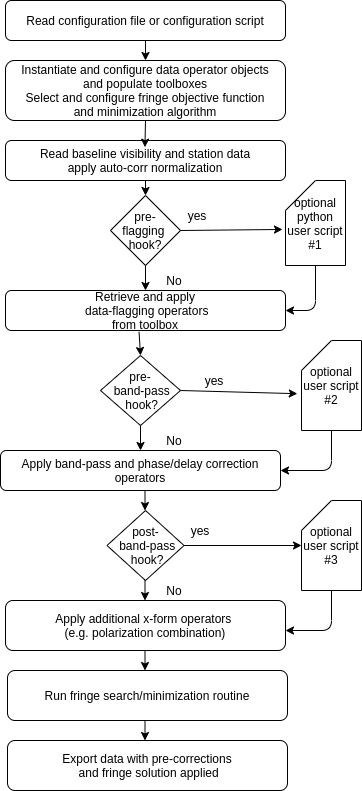
\includegraphics[width=0.6\textwidth]{fig/example-single-baseline-fringe-fitter.png}
    \caption{Example of simplified control flow for a single-baseline fringe fitter.}
    \label{fig:fringe-fitter}
\end{center}
\end{figure}

%%
% design details
%
\section{Commentary on Software Features and Design}
\label{sec:commentary}

The following sections provide some background and initial
design discussions for the topics listed in the outline.

\subsection{General Architecture}
\label{sec:genarch}

\subsubsection{Detail on language choice}
\label{sec:software-lang}
Several aspects need to be taken into account when deciding on a choice
of programming language for this project. Namely, some of these are:
\begin{enumerate}[itemsep=-1ex]
 \item Availability of software developer expertise.
 \item The inherent performance attainable with a specific language.
 \item Availability of high performance open source utility libraries
  for math, I/O, etc.
 \item The primary language of the existing code base (C).
 \item The accessibility and ease of extensibility of the project by
  users with varying levels of experience.
\end{enumerate}
Obtaining a reasonable balance between these considerations is difficult
with a single language. Therefore it may be desirable to consider a
multi-language project, wherein the base computation layer is handled
within C/C++, but additional data manipulation can be done via optional
Python plugins embedded within the appplication or independently by
external Python scripts which have access to some of the underlying
application libraries.  C++ is a reasonable choice given current
personnel, and the possibility of reuse of portions of the existing code
base in C. It also allows for the use of a wide variety of open source libraries, bot C
and C++ (not least of which is the built in standard library which provides
access to a wide collection of basic data types (strings, vectors, maps, etc) and
algorithms (searching, sorting, etc) which reduces the required amount
of maintenance of internal code and reliance on external libraries.
Further augmenting C/C++ libraries with inter-language
communication to Python can be done via a wide variety of mature tools
(ctypes, boost.Python, SWIG, etc.), and may increases the ease at which
outside users can augment the software.  Adopting C++ would allow a
easier path to memory management (currently handled rather painfully
in the existing HOPS code base).

Note that Python 2 is no longer supported, so to be clear, all new
development will be Python 3.

\subsubsection{Build system version control}
\label{sec:software-build}
We have a working SVN repository and the system is currently
built with autotools.
Do we want to continue using SVN or move to git?
Do we want to continue using autotools or migrate to cmake?
We can consider both, but there is no rush or a compelling
reason to do either, except perhaps for long term maintenance.

\subsubsection{Options for parallel processing}
\label{sec:software-parallel}

The existing fringe-fitting process is largely a data-parallel
process operating on individual baselines with no inter-process
communication. This lends itself easily to simple parallelism using
multiple independent processes (SPMD), which has been exploited
\cite{blackburn2019eht} to deal with the EHT data volume. However, this approach
eliminates the ability to simultaneously fit for global or station-based
parameters and requires multiple iterations in order to apply successive
calibration/corrections. Therefore, if some calibration tasks are to be
done simultaneously with fringe-fringe fitting, this will require both a
substantial architectural change from the current fitting algorithm, but
also necessarily reduce the degree of (simple) parallelism available. To
accommodate this, some parallel processing will have to be addressed
within the application. There several architectural options from which
to choose to provide support for differing levels of parallelism. A
limited table of these options is detailed in the following table:

\small
\begin{tabular}{|c|c|c|c|}
\hline
Name & Classification & Hardware Scalability & Effort \\ \hline
OpenCL/CUDA & SIMD & Single machine, CPU/GPU & Low-Medium \\ \hline
pthreads & MIMD & Single machine (CPU) & Medium \\ \hline
c++11 threads & MIMD & Single machine (CPU) & Medium \\ \hline
OpenMP & SIMD & Single machine (CPU) & Low-Medium \\ \hline
OpenMPI & MIMD & Multiple machines (CPU) & High \\ \hline
\end{tabular}
\normalsize

Note that a proper re-design of the data types and low-level algorithmic
codes should make it relatively straightforward to develop various
parallel versions of the fringe fitter or analysis tools, but this should probably be done
only after profiling a single-threaded version of the code, to determine where the most crucial
bottlenecks are.

\subsubsection{Interactivity vs. batch processing}
\label{sec:software-interaction}

The existing HOPS processing is batch-oriented for fringing, but
interactive at the \texttt{aedit} stage\dots.

Batch-oriented fringe production works well at the later stages (after
tuning) but at the initial analysis stages, some flexibility is needed.
This is particularly true as the amount of information contained in
broadband fringing greatly exceeds what will fit on one page.  And
expansion to multiple pages places more burden on the analyst---too
much to look at.

In the analysis stage (e.g. \texttt{aedit}) some degree of sophistication is
needed in the selection and display of data.  Again, the volumes of
data to be understood will require smarter software.

\subsection{External package dependencies}
\label{sec:software-externals}

In order to leverage existing open source software some decisions should be made relatively early on about which external (maintained by outside unrelated entities)
should be required. For example the current library used by HOPS for executing FFT's is FFTW3, which is required and not optional, likewise, for creating fringe
plots the package pgplot is required and not optional. Wherever possible requirements should be made optional in order to keep complexity low and reduce reliance on
external maintainers, but to make the best use of existing resources some minimal subset needs to be decided upon.

\subsection{Imports from Correlator Output}
\label{sec:corr-imports}

\subsubsection{DiFX Outputs}
\label{sec:difx-corr}

At present DiFX is the de-facto correlator for the EHT.  However, there
are other correlator codes (e.g. SFXC or CorrelX) that may be useful in
the future.  Also the so-called Swinbourne output format from DiFX may evolve.
Thus we need a define a suitably generic model for the correlation output
that will be adaptable to possible future development.

In general this framework includes inputs to the correlation (e.g.
VEX and V2D) as well as correlation setup files (e.g. calc).

\subsubsection{File conversions}
\label{sec:corr-import}

The current HOPS pathway from DiFX is difx2mark4 which is very specific
to DiFX and (the current) HOPS.  For analyis in AIPS or CASA, the difx2fits
program is currently used.

Aside from file input, there is generally a desire to migrate data
between the HOPS world and the AIPS/CASA world.  Thus it is sensible
to provide pathways from the new HOPS file structure to these other
tools.

\subsection{Exports to Subsequent Analyses}
\label{sec:exports}

\subsubsection{UVFITS}
\label{sec:uvfits}
The current C\&E-WG processing pipeline ends with the generation of
the UV flavor of FITS (UVFITS).  That tool should properly be updated
to work with the new fileset and added to the HOPS tool collection.

\subsubsection{CALCSOLVE}
\label{sec:calcsolve}
The geodetic analysts current take delivery of HOPS fringe results
for import into their CALCSOLVE program which solves for Earth Orientation
Parameters and other geodetic products.  The current delivery format is
native HOPS mk4 file format.  This capability must be preserved until
they can adopt their input library to use the new HOPS.

\subsection{HOPS file specifications}
\label{sec:hopsfiles}

\subsubsection{File Types}
\label{sec:ftypes}
HOPS makes use of a filesystem, and every file consists of representations
of objects.  A uniform plan for migrating these from what we currently have
to something more sensible is a project that decomposes into the various
types discussed in the next sections.  This design task consists of
all of the general considerations before the details of the subsequent tasks.

\subsubsection{Mark4 file types}
\label{sec:mk4types}
The existing ``Mark4'' filesystem was (believe it or not) an improvement
of the previous ``Mark3'' filesystem which was closely wedded to (a now
extremely outdated) filesystem for an HP filesystem.  The modularity of
the Mark4 data types is not particularly in question.  However the binary
format is bigendian and wedded to the C structures and other capabilities
of the UNIX system that was available at the time (SunOS, a precursor of
Solaris).  Since that time a number of viable archival data formats have
been created and are in general use.  A migration of the Mark4 types to
an HDF5-based fileformat is considered to be the desirable option at this
point.  The libraries from that package are well tested and essentially
ready to use.

\subsubsection{Python Wrappers}
\label{sec:pywrap}
One of the first steps of the C\&E-WG was to create Python wrappers for
the Mark4 types so that some manipulations could be done directly in
Python.  This is now considered an essential feature and it should be
natively supported by \nuHOPS.
\marginnote{\tiny{CASA uses numpy within its python layer, so that is
likely a component of our python user interface.  Since this was written,
I've discovered that SWIG may be used to automatically generate some of
the bindings, including for numpy, if one is judicious about what you ask
SWIG to do.}}

\subsubsection{Alist}
\label{sec:alist}
Following fringing, for the data analysis stage, HOPS provided a ``oneline''
fringe format (an aline) which could be manipulated by several tools
(e.g. \texttt{alist} and \texttt{aedit}).
The amount of information that is desirable to
be captured on the aline has grown to the point of incomprehensibility,
but the need for such a thing remains.  The precise solution is likely
a topic of study as there are a number of alternatives.

\subsubsection{Fourfit Control File}
\label{sec:control}
The fringing process may be controlled (almost) equivalently on the
command line or via a ``control'' file.  This file has a peculiar
format supporting a limited set of logic contructs for setting various
parameters.  In a package making specific use of Python, it is sensible
do discard the existing control file machinery in favor of a native
Python format and conventions for command line adjustments to it.

\subsubsection{VEX file parsing}
\label{sec:vex2xml}
The VLBI Experiments are specified in a rather arcane VEX file which
is currently stuck at verion 1.5.  The community has identified a version
2.0, but it has not actually been implemented.  For use at ALMA, we
developed and recently added to HOPS a VEX2XML parser that allows the
VEX file to be parsed to XML and then standard XML libraries may be
used to extract information.  We propose to adopt 2.0 features as they
become useful to the EHT, and work through the VEX2XML parser tool.

\subsection{New Objects}
\label{sec:newobjects}
The mark4 fileset stores data in number types:  the 100 series for
correlation products, the 200 series for fringes and the 300 series
for station calibrations.  The list grew in a somewhat ad hoc fashion
and was decidedly driving by the needs of analyzing data from the old
hardware correlator.  The list of types needs to be reviewed and
re-organized for the modern era.

\subsection{Algorithmic specifications}
\label{sec:algospecs}

\subsubsection{Baseline-based delay/delay-rate fitting}
\label{sec:fringing}
At the heart of fourfit is the baseline-based delay/delay-rate fitting.
Fourfit expresses as both a so-called ``single-band delay'' (SBD, an average
over the recorded channels) as well as the ``multi-band delay'' (MBD, over the
full band).  This algorithm must of course be preserved, but it should
be noted that it may be decomposed into the data calculations and the fitting
program.  The current algorithm also allows for an ionospheric fitter.
These parts must be decomposed and put in library functions for more flexible
use.

\subsubsection{Global Fringe Fitting}
\label{sec:globalfringe}
In particular, given a saner organization for the fitting, it should be
possible to provide the (more conventional, as provided in AIPS and CASA)
global fringe fitter which assigns results on a station basis.  This requires
a(t least one) least-squares fitting technique to be implemented.

\subsubsection{Spectral Line Fringing}
\label{sec:specline}
There are developments in mmVLBI that should allow work with spectral line
(i.e. narrow) sources; support for this capability should be in place in
the \nuHOPS.

\subsubsection{Ionospheric Fitting}
\label{sec:ionosphere}
VGOS currently fits for the total electron content (TEC) of the ionosphere
as part of the high-delay precision fits.  This is likely not needed at
the high frequencies the EHT uses, but it definitely must be preserved.

\subsubsection{Coherence Fitting}
\label{sec:cofit}
The current HOPS tool \texttt{cofit} allows one to identify the shortest
averaging interval with the maximum SNR.  The algorithm and plotting
artifacts should be continue to be supported as the tool is still useful.

\subsubsection{Weak Fringe Searching}
\label{sec:search}
The current HOPS tool \texttt{search} allows one to examine the two-dimensional
delay and delay-rate space to ascertain whether weak peaks are likely to be
real or not.  The tool is still of some use and should be retained.

\subsubsection{Pulsar Folding/Searching}
\label{sec:pulsar}
Support for folding data on a known pulsar period, or for searching
for pulsar periodicities in data was at one point contemplated for HOPS.
It may be useful to consider this in the new architecture.

\subsubsection{Space Based Support}
\label{sec:space}

If there is a future possibility of space based radio telescopes participating in the EHT network, this may require some additional features in the fringe fitting software, such
as compensating for higher order delay residual terms (delay-acceleration) in addition to the linear delay/delay-rate model used for ground based stations.

\subsubsection{PolConvert}
\label{sec:polconvert}
The ALMA observatory uses a linear, rather than a circular polarization
basis.  The current practice is to follow the correlation process (into
a mixed basis) by a polarization conversion step (using the tool
\texttt{PolConvert}).  In principle this step could be carried out in
the post-processing stage within \nuHOPS.  The architecture should
support this.

\subsection{Calibration Specification}
\label{sec:calspecs}

\subsubsection{Phase Calibration}
\label{sec:phasecal}
The EHT generally has used manual phase cals (no other alternative).
The geodetic sites generally have a pulsed tone phase cal system.
Depending on whether a pulsed system can be developed for the EHT,
it may in principal need to use both methods.

\subsubsection{Manual Phase Calibration}
\label{sec:manphasecal}
Lacking a pulse phase cal system at all of its observatories, the EHT
generally relies on a manual phase cal procedure.  There are several
scripts that have been written to estimate the manual phase cals (at
each station) on one bright scan and then place these phases into the
control file.  Likewise, delays may be estimated from a single scan
and placed in the control file.  Scripts to continue to do this must
be supported in the \nuHOPS~architecture.

\subsubsection{Pulse Phase Calibration}
\label{sec:pulsephasecal}

Pulse phase calibration is a method of compensating for the time varying phase and delay response of a telescope's receiving system. This is done
by injecting a train of sharp pulses (a Dirac comb) which are synchronized with the site's reference clock. This train of pulses is equivalent
to set of equally separated tones in frequency space. Since the tones are known to be in phase at the point of injection, it is then possible to monitor
the frequency dependent phase changes made to the incoming signal by the receiving system by tracking the accumulated phase of each tone.
This technique allows for the elimination of the (possibly time-varying) dispersion introduced by the receiving system.

Typically this calibration process is applied to the data in two steps after it is recorded. The first step is the extraction of the phase calibration tone phases. This is primarily done by
the correlator by calculating the in-phase and quadrature components of the stations' signals at each of the discrete tone frequencies. The second step is done during the fringe-fitting process,
where each stations tone-phase data is applied to correct the correlated signal. When there are many tone available across the correlated bandwidth, this process also allows for the correction of
instrumental delays (higher order terms are not currently considered). However, as is often the case, the pulse calibration data is not perfect and it can be significantly contaminated by RFI or weak tones.
The current implementation of (multiple tone) phase-calibration in fourfit is fairly robust, and admits some ability to mask bad tone data. However, there is ample room for improvement in the automatic
flagging of bad phase calibration data, which would be especially useful in the case where the data quality varies across both the time and frequency domain.


\subsubsection{Instrumental Bandpass Calibration}
\label{sec:bandpass}
It should be possible in \nuHOPS~to perform an instrumental bandpass
correction as is available in other packages.  Here one or more scans
on a bright calibrator may be used to establish the per-station deviation
of the bandpass from the optimal flat response.  These derived bandpass
solutions may then be applied to adjust the correlation amplitude as a
function of frequency.  Such a bandpass correction  may also be fully
complex (i.e. phase adjustments as well).

\subsubsection{Atmospheric Phase Calibration}
\label{sec:atmosphere}

The currently implmentation of fourfit allows from some limited ability to handle atmospheric phase calibration. Currently, this is done via the introduction of ad-hoc phases, which are applied independently from the formal fitting procedure for delay/delay-rate.
In the existing EHT calibration pipeline, these ad-hoc phases are estimated (after data-flagging and some bandpass correction have been applied) from data residuals after the fringe-fitting. The smoothed phase corrections estimated from the residuals
must then be exported to a ad-hoc phase file in order to be applied on the next pass. This process (while generic) is time consuming and requires the presence of a reference station with good SNR to the majority of stations in the network. Therefore, it
desirable to have a dedicated algorithm to estimate and apply atmospheric phase calibration within the fringe-fitting process itself.


\subsubsection{Polarization Calibration Corrections}
\label{sec:polarization}
In the current EHT analysis, network calibration techniques are used to self-calibrate the array for polarization work.  This is an area
to discuss with the other working groups what form of support in \nuHOPS~would be most effective. In addition, good estimates of station-based polarization calibration parameters
also enables the coherent summation (Stokes-I) of individual polarization-products resulting in higher SNR observations. This is also of great interest for geodetic observations, and important
for observations between stations with mixed polarization types (circular-linear).

\subsubsection{Ionopheric Calibration Corrections}
\label{sec:ionoscalcorr}

While the ionosphere does not typically play much of a roll at the high frequencies at which the EHT is observing (230, 345 GHz), knowledge of the ionosphere is crucial for obtaining
good results during geodetic observations that occur at lower frequencies (2-14 GHz) where the dispersion it causes is much stronger. Currently, fitting for the(line-of-site) differential total electron content ($\Delta$TEC) of the
ionosphere can currently be done from geodetic VLBI observations themselves during fringe-fitting on a single baseline. However, the current implementation could be strengthened if the fringe-fitting architecture were extended to allow for the possibility
of simultaneously fitting for the line-of-site TEC associated with station, as a station (rather than baseline) based quantity. This would help in the reduction of non-closing $\Delta$ TEC errors, and which can currently only be
done in an ad-hoc manner. Additionally, fitting for the $\Delta$TEC is sensitive to residual instrumental phase effects which can be difficult to detect unless examining data from multiple single baselines/scans.


\subsubsection{Source Structure Corrections}
\label{sec:sourcestructcorr}

One explicitly geodetic feature that may be desirable in the \nuHOPS is the possibility to introduce phase and delay corrections to compensate for source structure given an image model of a non-point like radio source. Having this ability would
eliminate a significant source of systematic error in geodetic delay observables, and allow for a larger catalog of usable (bright) sources for geodetic observations.



\subsection{Infrastructure}
\label{sec:infra}

\subsubsection{Messaging}
\label{sec:msg}
HOPS currently passes commentary to the user via a uniform messaging
service.  This allows the user to turn on verbosity or run completely
silently.  This should be preserved, but due to the potential volume
of such messages, the control should become finer grained---i.e. the
user should be able to specify what portions of code are making comments.

\subsubsection{Utilities}
\label{sec:utils}
HOPS has a few utilities for date or geometry calculations---these
should be reviewed and clearly supported.

\subsubsection{Performance}
\label{sec:perform}
HOPS has a performance monitoring system built into the existing code.
This should be retained and augmented by more sophisticated profiling tools.

\subsubsection{Averaging}
\label{sec:average}
Time averaging of data was added ad hoc to several of the tools; we
propose to build this capability in directly with native support.

\subsection{Data Inspection and Visualization}
\label{sec:inspect}

\subsubsection{To/From ASCII}
\label{sec:ascii}
Every bit of data that HOPS works with should be available in a human-readable
form.  So every object in the new design should support methods to export to
or import from some human readable format.

\subsubsection{The Fourfit Plot}
\label{sec:fplot}
The current fringe fitter, \texttt{fourfit} produces a single page summary
of the fringe result for every baseline.  In the high-bandwidth modern era,
one is hard pressed to capture everything in a readable format.  A single-page
format is still desirable, as is the ability to page through multiple plots
(i.e. as can be done with \texttt{fplot}), but some controls over the
information that is displayed is probably desirable.  Thus in \nuHOPS,
there will still be a standard page, but one may also create custom formats
which may be more useful for some experiment setups.

\subsubsection{Interactive Tools}
\label{sec:aedit}
The post-fringe processing in HOPS begins with \texttt{alist} which provides
one line summaries of every fringe.  These ``alist'' files may then be
used to make data-quality selections or support inspection (\texttt{fplot} of
errant fringes).  This capability must be retained, but it can almost certainly
be better implemented in Python, which would make it more extensible.

\subsubsection{Alternative Visualization}
\label{sec:alternatives}
Additional visualizations of data should be provided as these are often
useful for understanding subtle issues with data.  Again, a Python layer
providing access to the underlying \nuHOPS~data formats would probably be
the most elegant solution.

\subsection{New Libraries}
\label{sec:libes}
The existing algorithms should be encoded into new library methods
that have clear inputs, outputs and side-effects.  (In the current
HOPS, there are many side-effects to global variables, so the methods
cannot be directly reused as coded.)

\subsection{New Programs}
\label{sec:progs}
With the new architecture in place, versions of the existing programs
(e.g. \texttt{fourfit}, \texttt{alist} and \texttt{aedit}) should be
provided along with new, improved tools for the desired new capabilities.

%
% eof
%


\pagebreak


\section{Language, Build and Version Control System}
\label{sec:language}

Several aspects need to be taken into account when deciding on a choice of programming language for this project. Namely, some of these are:
\begin{enumerate}
 \item Availability of software developer expertise.
 \item The inherent performance attainable with a specific language.
 \item Availability of high performance open source utility libraries for math, I/O, etc.
 \item The primary language of the existing code base (C).
 \item The accessibility and ease of extensibility of the project by users with varying levels of experience
\end{enumerate}

Obtaining a reasonable balance between these considerations is difficult with a single language. Therefore we
plan to develop a multi-language project, wherein the base computation layer is handled within C/C++,
but additional data manipulation can be done via optional Python plugins embedded within the application
or independently by external Python scripts which have access to some of the underlying application libraries.
C++ is a good choice given current personnel and developer expertise, and being a super-set of the C language
it provides the ability to reuse of portions of the existing C code base with little to no change, while also adding modern language features
(templates, classes and inheritance, const. correctness, function overloading, etc.). A combined C/C++ approach
allows for much easier memory management (currently handled rather painfully in the existing HOPS code base) and also
enables the use of a wide variety of open source libraries, not least of which is the built in standard template library
which provides access to a wide collection of basic data types (strings, vectors, maps, etc) and algorithms (searching, sorting, etc.)
which will reduce the required amount of maintenance of internal code and reliance on external libraries.

Further augmenting C/C++ libraries with inter-language communication to Python can be done via a wide variety of mature tools
(ctypes, boost.Python, SWIG, pybind11, etc.), and will increase the ease at which outside users can augment the software without
needing to have expertise in C/C++/. Since Python 2 is no longer supported, all new development will be Python 3.

The build system for this project will be automake\urlfootnote{https://www.gnu.org/software/automake/} or CMake\urlfootnote{https://cmake.org}, and version control will proceed through a locally hosted (Haystack) git repository. HOPS3 used the automake build system and there is some
advantage in re-using that frame work, while the CMake build system is generally easier to maintain than the current automake system when faced with the complexities of a multi-language project. It also allows for a more user-friendly configuration at the time of compilation, as the user can be presented with a menu providing options which are dependent on the available set of tools/libraries that are currently installed and detected on the users system. Initialy
both build systems may be implemented to see which provides an optimal choice. While version control will be handled in a local \textit{git} repository during
the prime development phase, it is expected that eventually a public \textit{git} repository will be made available for releases which will also make it much easier to leverage community contributions if so desired at some point in the future.


\pagebreak

\section{Object specification}
\label{sec:objects}


Generally speaking the code will be organized around roughly three object type categories involved in the structure of the new HOPS. These are as follows:

\begin{enumerate}
 \item Meta Data Containers: These serve to store small quantities of station and baseline metadata associated with an observation of disparate types.
 \item Array Containers: These serve to organize large n-dimensional arrays of a single data type (e.g. visibility data and correction/calibration table data).
 \item Data Operators: These evaluate a function or perform some transformation on a given data container. Their operation is configurable via a set of externally defined parameters, while their application to any particular data set can be made conditional by a set of filters.).
\end{enumerate}

\subsection{Data Containers}

The existing HOPS3 code base relies on a fixed number of \texttt{C} structs to organize and present the data related to an observation. The strict memory layout of these structures has the advantage of making them cross-machine compatible, which is necessary since these structures are also used as the core components of the Mark-4 I/O library. However, a notable disadvantage of this rigid design is the degree of difficulty encountered in making changes to the existing data structures, or adding new data types in order to accommodate additional information which was not originally envisioned at the time the library was written. To make the data structures more flexible we intend to decouple the in-memory data layout from the file I/O, so they do not necessarily need to be byte-for-byte copies.

\subsubsection{Meta-Data Containers}

In a strictly typed language such as \texttt{C}, flexible data structures have a high degree of code overhead, not only in the management of dynamic memory allocation, but more severely in the conversion of data types and typecasting. To ameliorate this we propose to exploit \texttt{C++11}'s variadic template mechanism, which allows for the transformation of type-agnostic class lists into concrete class types or hierarchies at compile time. This makes it possible to store disparate types (so long as the complete set of types is known at compile time) within in the same object that are indexed and can be retrieved by the same type of key (e.g. a name string). Listing~\ref{lst:metaobjects} gives a condensed example of the preliminary version of the template base class for a meta-data container (with detailed functionality removed).

\lstinputlisting[language=C++,float=h!,label={lst:metaobjects},caption=Meta-data object template classes for multi-type maps.]{code/metadata-objects.hh}

To the extent possible, the in-memory meta-data structures should be classes which provide access via a key-value pair mechanism so as to avoid exposing the private internal storage layout to the routines needing access to subsets of the data. This retrieval mechanism also has the benefit of completely decoupling the compile
time structure of the data containers from the data they need to hold at runtime. A key:value interface is trivially available via the STL std::map template class,
so there is no need to expend effort on a native implementation. Moreover this sort of interface should also make conversion of these data structures into widely accessible formats such as JSON or python dictionaries possible for data export to external software.

\subsubsection{N-Dimensional Array Containers}

We propose the following basic set of class templates be used to construct most in-memory objects used for the manipulation of correlated observation data and its associated station data:
\begin{enumerate}
 \item \texttt{MHO\_ScalarContainer} - encapsulates scalar-like data
 \item \texttt{MHO\_VectorContainer} - encapsulates vector-like data
 \item \texttt{MHO\_TableContainer} - encapsulates rank-N tensor-like data with associated axes (vector)
\end{enumerate}
These template classes are to serve as a simple wrapper around the management of the raw memory needed to store a data item and keep track of its associated unit(s), and (if applicable) the values associated with the axes along each dimension and their units.

The three container types listed above represent the majority of the memory intensive data needed within HOPS
and can largely be derived from a N-dimensional array of some numeric or integral type. Therefore a generic template class for
N-dimensional arrays is needed, listing \ref{lst:ndarray} shows a stub of this class.
\lstinputlisting[language=C++,label={lst:ndarray},caption=N-Dimensional Array Template]{code/MHO_NDArrayWrapper.hh}
The underlying storage of the N-dimensional array data is done as a single contiguous chunk of memory which can either be a piece of externally or internally managed memory. Indexing into this chunk of memory is done using C-like row-major order, where for an array of rank D, with dimension sizes $\{N_0, N_1, \cdots N_{D-1}\}$, the location of the data specified by the indexes $\{n_0, n_1, \cdots, n_{D-1}\}$ can found at an offset from the start, $z$, that is given by:
\begin{equation}
 z = \sum_{k=0}^{D-1} \left ( \prod_{j=k+1}^{D-1} N_j \right) n_k
 \end{equation}
Access to the underlying data stored within a class of this type can then proceed in two main ways. The first is through the aforementioned
row-major order indexing operation, and the second is through the use of iterators. An example of several of the provided methods is shown for a three dimensional array in listing \ref{lst:array-usage}. Iterators are most commonly utilized for efficient incremental (continuous or strided) access to the array data as they can be computed using pointer arithmetic, while random access is best done via indexes.
\lstinputlisting[language=C++,label={lst:array-usage},caption=N-Dimensional Array access]{code/array_use.cc}

In addition to the raw data stored in the N-dimensional array, in the case of the \texttt{MHO\_TableContainer} it is important to associate a coordinate axis with each dimension in order to provide various data operators with the ability to look-up the location of a datum beyond a simple integer-index. To enable this,
we will pair an N-dimensional array with a tuple of axis objects associated with each dimension. Listing \ref{lst:objects} shows the template class structure
for a TableContainer (along with other) objects.
\lstinputlisting[language=C++,float=h!,label={lst:objects},caption=Data object templates]{code/data-objects.hh}
The axis objects themselves also inherit from \texttt{MHO\_IntervalLabelTree}, which provides the ability to associate a pair of indexes with a key value pair of several types. A simple example of this would be tagging a section of the frequency axis with a particular channel ID (e.g \texttt{ [0, 32] } $\leftrightarrow$ \texttt{ \{"channel\_id": "X17LY"\} }). The class \texttt{MHO\_IntervalLabelTree} will support tagging axis intervals with values of at least the following types: char, bool, int, double, and string, using strings as keys, and allow for the bi-directional look up of a key:value pairs with assoiated intervals.

As a concrete example of the \texttt{MHO\_TableContainer} template class, listing \ref{lst:visib} gives a simple example of what template declaration of an object storing channelized visibility data from a single-baseline observation might look like.
\lstinputlisting[language=C++,float=h!,label={lst:visib},caption=Visibility object type]{code/visibilities.hh}
For example, in the case of channelized visibilities, the axes of each of the four dimensions would be:
\begin{enumerate}
\item Axis 0: Polarization-product axis, labelled by a short string specifying the reference
and remote stations' polarizations for data associated with that column (e.g ``XX'' or ``RR'' or ``RX'').
\item Axis 1: Channel axis, labelled by a character or numerical value (e.g. ``A'' or 1).
\item Axis 2: Time axis, labelled by the time since start of a scan in seconds.
\item Axis 3: Frequency axis, labelled by the frequency offset from the edge of the channel (MHz).
\end{enumerate}
It should be noted that these coordinate axes are there merely to label the data, but are not meant to provide a reverse look-up
capability, (e.g example inverting the polarization-product code ``LL'' to infer a 0-th index location of 0). For efficiency array
access should still be done using unsigned integer index values. A graphical representation of a \texttt{MHO\_TableContainer} is
shown in Figure~\ref{fig:table-container}.

\begin{figure}[h!]
  \begin{center}
  \captionsetup{width=0.7\linewidth}
  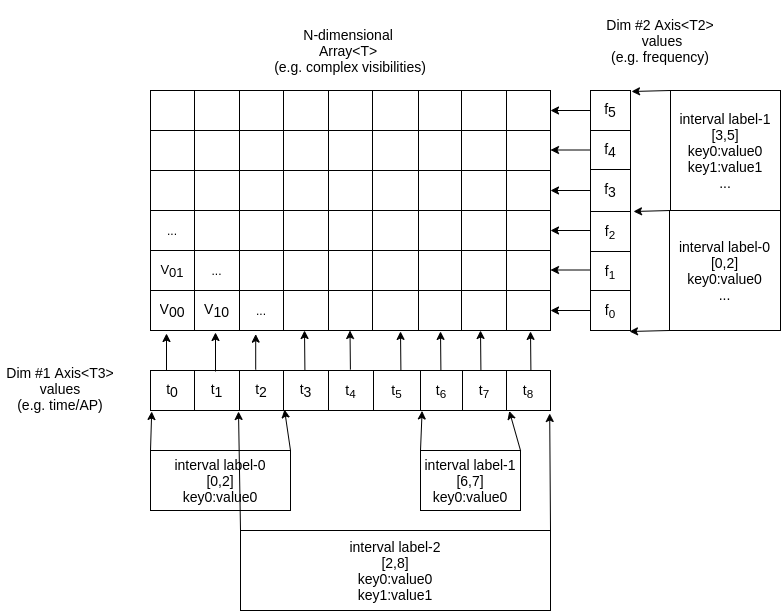
\includegraphics[width=0.75\textwidth]{fig/data-container-baseline.png}
    \caption{A graphical representation of a \texttt{MHO\_TableContainer}. This class is composed of an N-dimensional array, coupled with axes to provide coordinate values along each dimension. The axes themselves allow for arbitrary intervals to be labelled by key:value pairs in order to allow for local look-up of filter data. For example, along the frequency axis, the interval labels may be channel or sampler names among other possibilities. Furthermore, the interval and associated labels will be stored in an interval-tree structure to allow for fast bi-directional lookup of data indices $\leftrightarrow$ data labels.}
    \label{fig:table-container}
\end{center}
\end{figure}

\subsubsection{Specific data types}

Below is an incomplete table of the various data objects that are constructed from \texttt{MHO\_TableContainer}, along with their data value type and axis names. These may be subject to change (for example, \texttt{uint64\_t} may be unecessarily large for the flags type, and could be reduced).
\begin{center}
\resizebox{\textwidth}{!}{
\begin{tabular}{| c | c | c | c |}
\hline
 Name & value type & N-Dim & Axes \\  \hline
 Visibilities & \texttt{std::complex<double>} & 3 & (pol. product, time, frequency) \\ \hline
 Weights & \texttt{double} & 3 & (pol. product, time, frequency) \\ \hline
 Flags & \texttt{uint64\_t} & 3 & (pol. product, time, frequency) \\ \hline
 Channelized Visibilities & \texttt{std::complex<double>} & 4 & (pol. product, channel, time, frequency) \\ \hline
 Channelized Weights & \texttt{double} & 4 & (pol. product, channel, time, frequency) \\ \hline
 Channelized Flags & \texttt{uint64\_t} & 4 & (pol. product, channel, time, frequency) \\ \hline
 (static) per-Channel phase corrections & \texttt{double} & 2 & (pol. product, channel) \\ \hline
 Channelized Ad-hoc phases/amplitude corrections  & \texttt{std::complex<double>} & 4 & (pol. product, channel, time, frequency) \\ \hline
 \end{tabular}
 }
\end{center}

\subsection{Data operators}

The data operator classes are meant to organize the mathematic manipulations which are to be performed on the data containers. For example, many of the operations performed in the existing HOPS3 code-base (such as the application of a priori phase calibration) are relatively trivial linear transformations applied to the visibility data. However, they are currently intertwined with a large amount of control logic which obscures the basic data pathway (e.g see postproc/fourfit/norm\_fx.c)

Most unary or binary operations that are to applied to visibility or other data residing in an \texttt{HO\_TableContainers} such as scaling, multiplication, transposition, summation, Fourier transformation, etc. will be made available as individual classes inheriting from the same interface. A uniform class interface will allow these data operators to be composed or modified to create more complicated composite operators or strung together and called in an ordered fashion in order to accomplish data pipelines of arbitrary complexity. An additional advantage of encapsulating individual operations is that (coupled with the data container extensions) any SIMD parallel-processing extension used to accelerate data processing can be made opaque to the user.

Listing \ref{lst:operators} gives a brief sketch of the class templates generalizing the data operators. The common inheritance from the base class \texttt{MHO\_Operator} allows them all to be stored in an common container (e.g. \texttt{std::vector<MHO\_Operator*>}) so that once they are
constructed and configured they may be retrieved and intialized/executed in the appropriate order. Listing \ref{lst:operator-use} shows a brief code
sketch demonstrating how two simple operators would be constructed, assigned arguments and then initialized and executed in order.

\lstinputlisting[language=C++,float=h!,label={lst:operators},caption=Data operator template classes.]{code/operator_use.cc}

It is expected that the vast majority of the data operators will be unary or binary, requiring only their own configuration parameters along with one or two data containers upon which they operate as inputs. 
However, any number of arguments is possible so long as the underlying implementation provides the appropriate overload.

One aspect of the data operators which is not yet detailed here is a notion of what pieces of meta-data each operator may need in order to complete its function. 
Some of the more primitive operations (e.g. complex conjugation) may not need any meta-data, while certain 
specific calibration routines may need station related meta-data (e.g. channel specific phase-cal).
While some meta-data items could be exposed directly via external setter/getters, a possibly preferable option which would preserve encapsulation might be for each operator to define an internal schema, 
listing the keys and type of the parameters it needs to retrieve from a single meta-data container (populated from the vex), or what sort of labels it expects to be attached to the data containers on which it operates.
In addition, a mechanism for filtering operations (e.g. if station = Xx, then apply this operator) also needs to be established independent of the previous control-block structure of HOPS3.

\lstinputlisting[language=C++,float=h!,label={lst:operators},caption=Data operator template classes.]{code/data-operators.hh}

\subsubsection{Specific data operations}

Below is an incomplete list of various data operations. A full specification of each operation is detailed in the subsequent pages.
\begin{enumerate}
 \item MHO\_ComplexConjugator: Apply a complex conjugation to all elements of an ND-array.
 \item MHO\_CyclicRotator: Apply a cyclic rotation to the selected axes of an ND-array.
 \item MHO\_FastFourierTransform: Apply a Fourier transform to a one dimensional array.
 \item MHO\_FunctorBroadcaster: Apply a specified unary function to each element of an ND-array.
 \item MHO\_MultidimensionalFastFourierTransform: Apply a Fourier transform to the selected axes of an ND-array using native libary.
 \item MHO\_MultidimensionalFastFourierTransformFFTW: Apply a Fourier transform to the selected axes of an ND-array using FFTW library.
 \item MHO\_MultidimensionalPaddedFastFourierTransform: Apply a zero-padded Fourier transform to the selected axes of an ND-array.
 \item MHO\_Reducer: Apply a reduction (e.g. sum all elements) along the selected axis of an ND-array.
 \item MHO\_SubSample: Skip select every n-th element of an ND-array for a specified axis of a ND-array.
\end{enumerate}

\newpage

\noindent \textbf{Name:} MHO\_ComplexConjugator \\
\textbf{Type:} Unary, in-place and out-of-place (requires copy). \\
\textbf{Template Parameters:} The specific N dimensional array type.\\
\textbf{Configuration Parameters:} None.\\
\textbf{Inputs:} A N dimensional array with complex double/float value type. \\
\textbf{Outputs:} A N dimensional array with complex double/float value type. \\
\textbf{Description:} Iterates over all values in an N dimensional array and applies the operation \texttt{std::conj()} to each element, according to algorithm \ref{algo:complex-conjugator}. \\


\begin{algorithm}[h!]
  \caption{Complex conjugation operator.}
    \begin{algorithmic}[1]
    \Require{Complex array $\mathbf{X}$ of rank $N$, and total size $M$.}
	\State {\textbf{for} $j=0\ldots M$ \textbf{do} }
	\State {$\quad \mathbf{X}[j] = \overline{\mathbf{X}[j]}$ }
    \State{\textbf{return}.}
    \Ensure{Conjugate array, $\overline{\mathbf{X}[j]}$.}
    \end{algorithmic}
  \label{algo:complex-conjugator}
\end{algorithm}


\noindent \textbf{Name:} MHO\_CyclicRotator \\
\textbf{Type:} Unary, both in-place and out-of-place. \\
\textbf{Configuration Parameters:} Requires the integer index of the axis to be rotated, and the integer offset specifying the size of the rotation. A positive value of the rotation offset results in a right shift cyclic rotation, while a negative value results in a left shift cyclic rotation.\\
\textbf{Inputs:} A N dimensional array with arbitrary trivially copyable type. \\
\textbf{Outputs:} A N dimensional array with arbitrary trivially copyable type. \\
\textbf{Description:} Performs cyclic rotation upon the requested axis for the specified offset, according to algorithm \ref{algo:cyclic-rot}.

\begin{algorithm}[h!]
  \caption{Cyclic rotation operator.}
    \begin{algorithmic}[1]
    \Require{Array $\mathbf{X}$ of rank $N$, with dimensions of $\{n_1, n_2, \ldots, n_{N-1} \}$ and total size $M$, and the integer offsets of each axis to be rotated $m_i$.}
	\State {\textbf{for} $j=0\ldots M $ \textbf{do} }
    \State {$\quad$ Compute the indices $\{k_0, k_1, \ldots, k_{N-1} \}$ associated with location $j$.}
    \State {$\quad$ \textbf{for} $i=0\ldots N-1$ \textbf{do}  $k'_i = k_i + m_i \;\; \mathbf{mod} \;\; n_i$. }
	\State {$\quad \mathbf{Y}[k'_0, k'_1, \ldots, k'_{N-1} ] = \mathbf{X}[k_0, k_1, \ldots, k_{N-1}]$ }
    \State {\textbf{return}.}
    \Ensure{The rotated array $\mathbf{Y}$.}
    \end{algorithmic}
  \label{algo:cyclic-rot}
\end{algorithm}



\noindent \textbf{Name:} MHO\_FastFourierTransform \\
\textbf{Type:} Unary, both in-place and out-of-place. \\
\textbf{Configuration Parameters:} Requires the direction of the transform to be specified (forward/backward), the direction follows the convention of FFTW.\\
\textbf{Inputs:} A one dimensional array with complex double/float value type. \\
\textbf{Outputs:} A one dimensional array with complex double/float value type. \\
\textbf{Description:} This operator performs an Fourier transform (or inverse transform) on the input array using an FFT algorithm. If the array size is a power of two, then either a Cooley-Tukey or Gentleman-Sande radix-2 algorithm will be applied. For all other sizes, the Bluestein/Chirp-Z algorithm is used.\\



\noindent \textbf{Name:}  MHO\_FunctorBroadcaster \\
\textbf{Type:} Unary, both in-place and out-of-place. \\
\textbf{Configuration Parameters:} The unary functor class to be applied to each element of the array (this is a template parameter).\\
\textbf{Inputs:} A N dimensional array with any value type (must be acceptable to the functor)\\
\textbf{Outputs:} A N dimensional array with any value type (must be acceptable to the functor)\\
\textbf{Description:} For every element in the array the functor operation will be applied, in the case of an out-of-place operation a copy will take place.\\


\noindent \textbf{Name:} MHO\_MultidimensionalFastFourierTransform \\
\textbf{Type:} Unary, both in-place and out-of-place. \\
\textbf{Configuration Parameters:} The indices of the dimensions which are to undergo transformation(default is all), as well as direction of the transform to be specified (forward/backward), the direction follows the convention of FFTW.\\
\textbf{Inputs:} A N dimensional array with complex double/float value type \\
\textbf{Outputs:} A N dimensional array with complex double/float value type \\
\textbf{Description:} Executes a Fourier transform on the selected dimensions of the array using the native FFT calculator.\\


\noindent \textbf{Name:} MHO\_MultidimensionalFastFourierTransformFFTW \\
\textbf{Type:} Unary, both in-place and out-of-place. \\
\textbf{Configuration Parameters:} The indices of the dimensions which are to undergo transformation (default is all), as well as direction of the transform to be specified (forward/backward), the direction follows the convention of FFTW.\\
\textbf{Inputs:} A N dimensional array with complex double/float value type \\
\textbf{Outputs:} A N dimensional array with complex double/float value type \\
\textbf{Description:} Executes a Fourier transform on the selected dimensions of the array using the FFTW library, the precise algorithm selected is determined by FFTW.\\


\noindent \textbf{Name:} MHO\_MultidimensionalPaddedFastFourierTransform \\
\textbf{Type:} Unary, both in-place and out-of-place. \\
\textbf{Configuration Parameters:} The indices of the dimensions which are to undergo transformation (default is all),
the padding factor $M$ and the direction of the transform (forward/backward). The zero padding can be specified as either symmetrically center padded (zeros place in middle of array), or end-padded.\\
\textbf{Inputs:} A N dimensional array with complex double/float value type with even lengths in each dimension to be transformed. \\
\textbf{Outputs:} A N dimensional array with complex double/float value type with even lengths in each dimension to be transformed.\\
\textbf{Description:} For each selected dimension of length $n$, the array will be padded with zeros, such that the new length will be $nM$. The zeros will either be placed in the center of the re-sized array (center-padded), or at the end (end-padded). The resulting padded array will then be transformed using the native FFT calculator. The primary use case of this padded FFT is for interpolation.\\


\noindent \textbf{Name:} MHO\_Reducer  \\
\textbf{Type:} Unary, both in-place (requires copy and resize) and out-of-place. \\
\textbf{Configuration Parameters:} The indices of the dimensions which are to undergo reduction, and the operation which is to execute the reduction (addition or multiplication). \\
\textbf{Inputs:} A N dimensional array with numerical value type\\
\textbf{Outputs:} A N dimensional array with numerical value type\\
\textbf{Description:} The input array will be reduced along the selected axes, and depending on the operation (addition or multiplication), the contents will be resized and replaced by the sum or product of the elements along that axis.\\

\noindent \textbf{Name:} MHO\_SubSample  \\
\textbf{Type:} Unary, both in-place and out-of-place. \\
\textbf{Configuration Parameters:} The index of the dimension along which the sub-sampling operation should take place, and the stride at which elements are re-sampled.\\
\textbf{Inputs:} A N dimensional array with any value type\\
\textbf{Outputs:} A N dimensional array with any value type\\
\textbf{Description:} For a stride value of $k$, and dimension index $j$, the output array will be resized and populated in such a way that only every $k$-th element (along the $j$-th dimension) from the original array will remain.\\



\subsubsection{Data Container Extensions}

The primary goal of the containers is to provide a relatively simple and efficient representation of commonly used data types that hides the details of
memory management and array indexing/access from the user. They should not be overburdened with too much extraneous functionality that is specific to a particular operation that must be executed upon them as this greatly
over complicates these classes and makes them brittle. 

However, there are some cases where this sort of decoupling may induce a performance cost. An example of
this occurs in the case of SIMD/GPU acceleration. In order to make use of GPU processing the data must be copied to a buffer on the device, processed, and then the results must be passed back to the host. However, if there are several operations to be performed in succession on the GPU, only first and last transfer need to occur, with intervening transfers being unecessary as input data is already present on the device. However, in order to eliminate the intermediate transfers a handle to the device buffer must be kept persistent in memory. So the questions arises, where should we keep this device buffer object? Should it be kept as a member of the data operator? That would be a poor choice, since if it is private it will not accesible to other operators to make use of, and if it is public then it will introduce the possibility of tight coupling with other portions of the code making use of the buffer. On the other hand, a pointer to a device buffer is too specific to belong in something as basic as a data container. However, it is a good candidate for something to may be stored in an extension.

In order to provide the ability to append extensions to the data containers, they must all inherit from a base class, \texttt{MHO\_ExtensbleElement}, which
in turn stores a vector of type-erased\footnote{https://davekilian.com/cpp-type-erasure.html} pointers to the extensions themselves. The extensions are templated on the the class providing the additional functionality and must all inherit from the base class \texttt{MHO\_ExtendedElement} (so they can be stored in the vector owned \texttt{MHO\_ExtensbleElement}) A brief sketch of the code that allows for this is shown in listing \ref{lst:extend}. One draw back of this method is that requires $N$ \texttt{dynamic\_cast} calls any time a particular extension is modified or accessed via the data container. 
This is an acceptable trade off for infrequent access to expensive (to construct) extensions, but should be used rather sparingly as \texttt{dynamic\_cast} has high overhead.

\lstinputlisting[language=C++,float=h!,label={lst:extend},caption=Data container extension classes.]{code/MHO_ExtensibleElement.hh}

%%
%  Annotated source tree; regenerate the list with
%
%   find . \( -name .git -o -name cmake -o -name m4 -o \
%             -name auto\* -o -name src -o -name lib -o \
%             -name include \) -prune -o -type d -print
%

\section{Annotated Source Tree}
\label{sec:srctree}

\FIXME[need a python script to do the find, or similar and re-generate
appropropriate section headings]

\tiny
\begin{verbatim}
./doc
./doc/covertest
./doc/common
./doc/developer
./doc/develplan
./doc/reference
./doc/userman
./doc/code_outline
./doc/geodetic
./doc/requirements
./doc/specification
./doc/specification/code
./doc/testreports
./source
./source/c_src
./source/c_src/mk4util
./source/c_src/afio
./source/c_src/applications
./source/c_src/applications/alist
./source/c_src/applications/aedit
./source/c_src/applications/fourfit
./source/c_src/dfio
./source/c_src/vex
./source/c_src/vex/text
./source/c_src/fourfit_libs
./source/c_src/fourfit_libs/ffplot
./source/c_src/fourfit_libs/ffsearch
./source/c_src/fourfit_libs/ffcontrol
./source/c_src/fourfit_libs/ffcore
./source/c_src/fourfit_libs/ffio
./source/c_src/fourfit_libs/ffmath
./source/python_src
./source/python_src/scripts
./source/python_src/hops
./source/bash_src
./source/cpp_src
./source/cpp_src/Messaging
./source/cpp_src/MK4Interface
./source/cpp_src/Bindings
./source/cpp_src/Utilities
./source/cpp_src/Test
./source/cpp_src/Containers
\end{verbatim}



\pagebreak

\section{Parallel processing}
\label{sec:parallel}

The existing fringe-fitting process is largely a data-parallel process operating on individual baselines with no inter-process
communication. This lends itself easily to simple parallelism using multiple independent processes (SPMD), which has been exploited
\cite{blackburn2019eht} to deal with the EHT data volume. However, this approach eliminates the ability to simultaneously fit for global or station-based
parameters and requires multiple iterations in order to apply successive calibration/corrections. Therefore, if some calibration tasks are to be
done simultaneously with fringe-fringe fitting, this will require both a substantial architectural change from the current fitting algorithm, but
also necessarily reduce the degree of (simple) parallelism available. To accommodate this, some parallel processing will have to be addressed
within the application. To do this we will use a multi-staged approach during the course of development.

Initially, the software to be developed under this project will focus on a simple single-threaded implementation, whereupon careful
profiling will inform us of the largest computational bottlenecks. For example, in the current HOPS code the majority of
the computation time is spent in a single routine (vrot.c, which is essentially just evaluating a complex exponential and multiplying two complex numbers) that is applied over
a large array of data. This sort of task can easily be parallelized on modern multi-core architectures using the SIMD approach. We propose to use OpenCL
for this purpose given its support on a wide variety of architectures (multi-core CPUs, GPUS, hardware accelerators, etc.).

OpenCL extensions for various data operations will be inherit from the operator templates described in listing \ref{lst:operators} and make use of the data container extension mechanism described in \ref{lst:extend}. This will allow them to function as drop-in replacements for single-threaded operators (in use within compound operators) that can be enabled when the underlying hardware is present. For example, lets consider the task of performing a scaling operation on a large array. Normally, this is trivially implemented in single-threaded fashion with a simple for-loop. However, OpenCL can be exploited to apply the scale factor across large chunks of the array in parallel. To do this, a container object is first extended with an OpenCL buffer object (by the operator). The device buffer is then populated with the host data and the SIMD implementation of the data operation is executed by the device. If desired, the results can be transferred back to the host, or can remain on the device side buffer for immediate use if the next operation also happens to be an OpenCL enabled operator. This process is all hidden behind the public interface of the data operators (listing \ref{lst:operators}) using (\texttt{SetArgs(...)}, \texttt{Initialize(...)}, and \texttt{Execute(...)}, so SIMD enabled operators and standard single-thread operators can be made interchangeable.


SIMD parallelism exploits vector instructions and/or multiple processors to execute the similar operations over wide swaths of data. While given current experience with the existing HOPS leads us to expect that SIMD parallelism should largely be adequate to accelerate fringe fitting, if during the process of development it is discovered that a thread-based model (MIMD, where each parallel thread follows a semi-independent code pathway) could be more advantageous, then we propose to use OpenMPI framework to implement this. The reason being, that while OpenMPI does have a larger development overhead than most other threading libraries (e.g. pthreads, c++11 threads, etc.) it can be easily scaled beyond a single computer when and if needed. However, it should be noted that by necessity, any OpenMPI implementation must be developed as an independent executable (although it would also be able to take advantage of any available libraries and SIMD policies present if the underlying hardware supports it). 


\pagebreak

\section{External Package Selection}
\label{sec:externals}

To the extent possible the software to be developed in this project should make all external dependencies optional whenever possible. That is to say, that
while some features may be missing if an optional external package is missing, the core functionality of the software should not be affected. For example, if the fast Fourier transform library FFTW3 is missing, the code should fall back to an internal implementation (which is allowed to be slower), but which produces equivalent output. Likewise, while an effort should be made to support portability of the output data into useful downstream formats (HDF5), this should not preclude a
basic native format capable of storing the same data for fallback, development, and debugging purposes.

The following table is a preliminary list of which external packages are expected to be incorporated as required or optional dependencies. If an optional package is missing on a user's machine the software will default to a fallback option (if available) or disable the features which require that particular package.

\begin{center}
\begin{table}[h!]
\begin{adjustbox}{width=\textwidth}
\begin{tabular}{|c|c|c|c|}
\hline
Name & Optional/Required? & Purpose & Fallback option \\ \hline
C++11 STL & Required & Standard template library & None \\ \hline
Python &  Required & Scripting language interpreter & None \\ \hline
SWIG or pybind11 & Required & C/C++ $\leftrightarrow$ Python interface and bindings & None \\ \hline
OpenCL & Optional & SIMD parallelism & Single-threaded implementation \\ \hline
OpenMPI & Optional & MIMD parallelism & Single-thread implementation \\ \hline
FFTW3 & Optional & fast Fourier transform acceleration & native code \\ \hline
GSL & Optional & Linear algebra and special functions & TBD native code \\ \hline
HDF5 & Optional & File input/output & TBD native binary format \\ \hline
matplotlib & Optional & Python plotting library & None \\ \hline
difxio & Required & DiFX I/O library - needed for file converter only & None \\ \hline
\end{tabular}
\end{adjustbox}
\caption{List of optional/required dependencies.}
\label{tab:dep}
\end{table}
\end{center}


\pagebreak

\section{Interactivity and Interfaces}
\label{sec:interfaces}

Interactivity with the user will proceed primarily through a python scripting interface. This avoids the need to develop a separate scripting language, 
as the python interpreter can be embedded in the application. Access to library objects will be exposed via python bindings, so that a user may have direct access 
to the data containers and operators, and can implement external routines to modify the data. Real-time interactivity via CLI or GUI is 
not planned to be implemented. We intended to preserve the functionality of the existing \texttt{fourfit} control file input method, however, this
is primarily for backwards compatibility and regression testing, no new features will be made available via this mechanism.


\pagebreak

\section{Plotting Functions}
\label{sec:plotting}

The fringe fitting procedure in HOPS3 is tightly coupled with plotting, which is handled through PGPLOT. PGPLOT has been unsupported for many years and it will not be a required dependency in \nuHOPS. In \nuHOPS, fringe-fitting and plotting will be decoupled (fringe results can be generated and saved, with or without generating a plot), and the native plotting functions will be replaced with new code. We have prototyped a set of Matplotlib functions that reproduce the standard ``fringe'' plot generated by fourfit (see Figure~\ref{fig:matplotlib-fringe-plot}).

\begin{figure}[h!]
  \begin{center}
    \captionsetup{width=0.6\linewidth}
    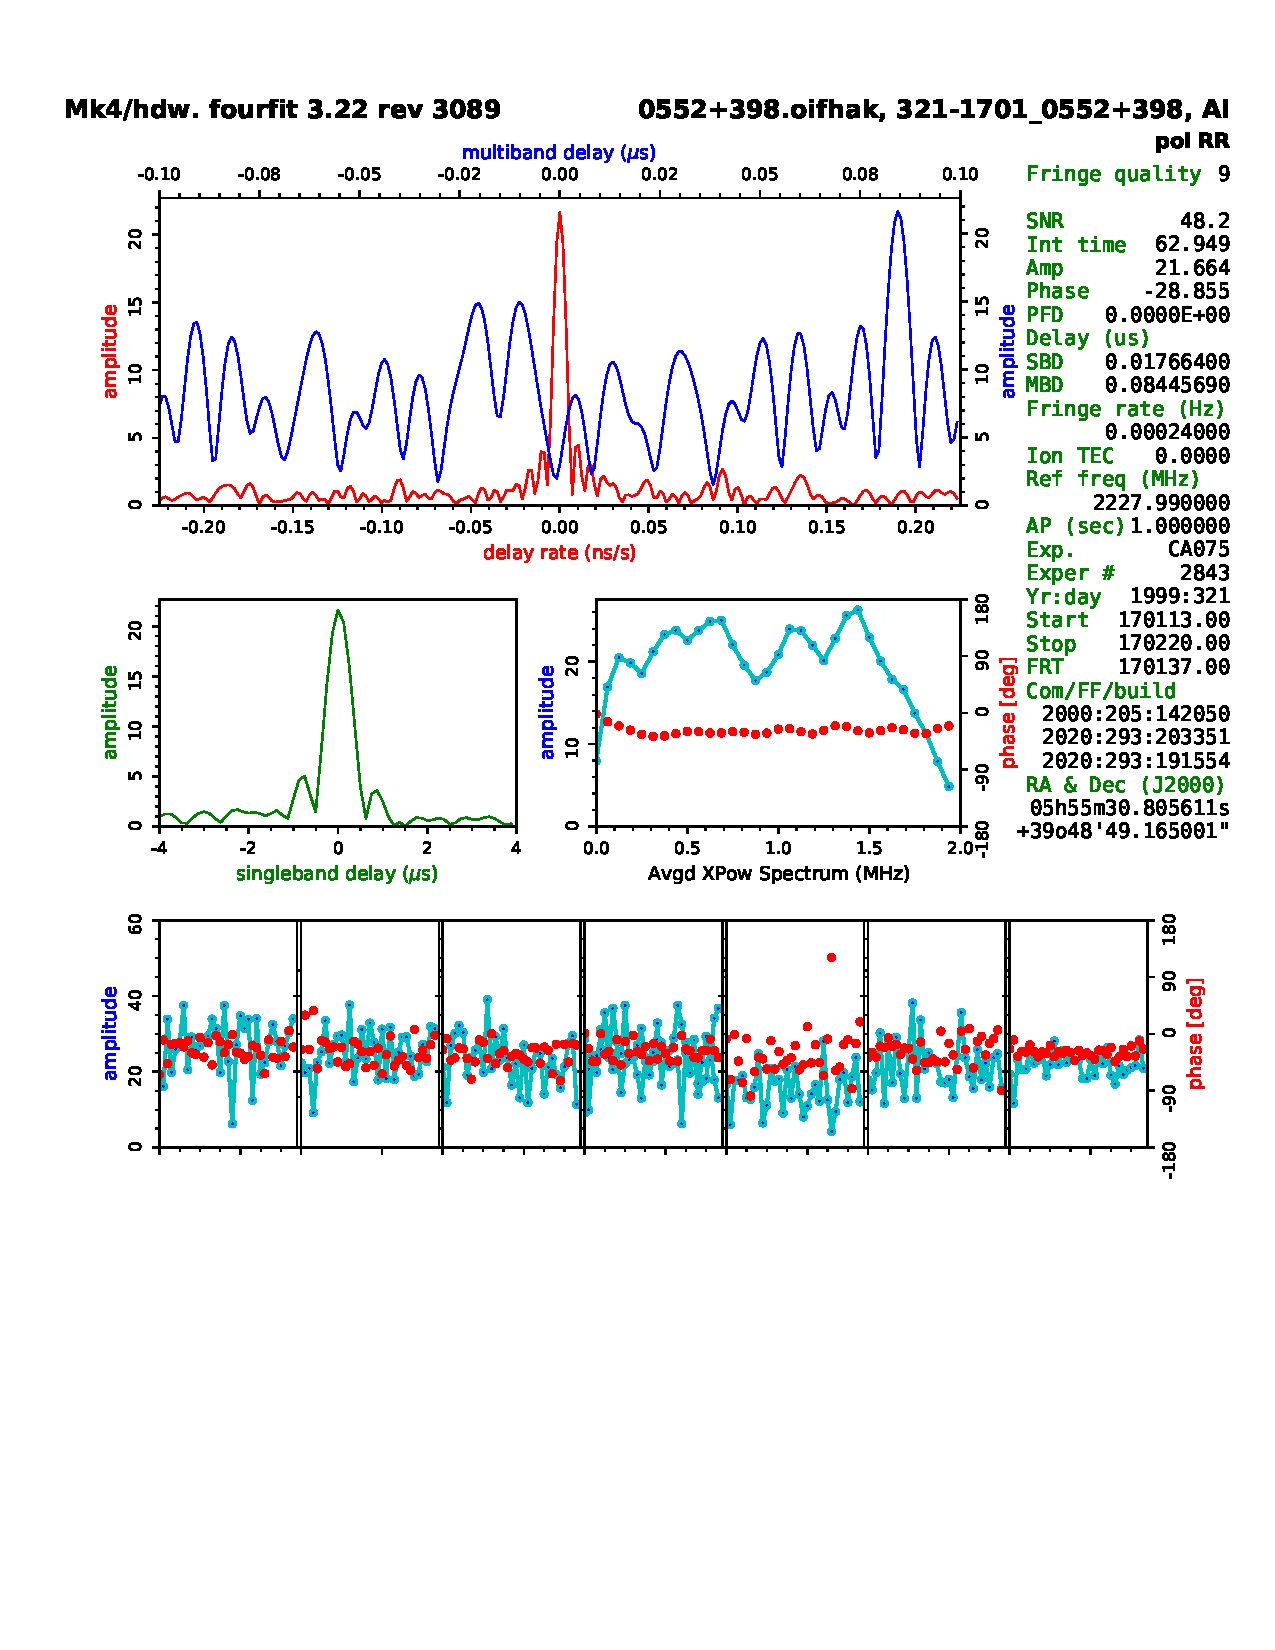
\includegraphics[width=0.7\textwidth]{matplotlib-fringe-plot.pdf}
    \caption{Example of a fringe plot with Matplotlib.}
    \label{fig:matplotlib-fringe-plot}
\end{center}
\end{figure}


The plotting functions of \nuHOPS will be expanded, and will include hooks for users to insert their own plotting functions, interactive plots for reformatting, and simple extensibility to add features.


\pagebreak

\section{Libraries and executables}
\label{sec:libraries}

\subsection{Libraries}

The libraries of this project are currently broken down by task into the following modules:

\begin{enumerate}
     \item Utilities - Commonly used utilities (e.g. date handling, profile timers, etc.)
     \item Math - Math routines: linear algebra, minimizers, interface to optional 3rd-party math libraries (FFTW,GSL).
     \item Message - Controls the topic and verbosity level of application messages/logs to user.
     \item Containers - In-memory data containers of visibility and meta-data and native format I/O.
     \item MK4Interface - Allows for import/export to legacy MK4-types for testing and backwards compatibility.
     \item Operators - Base classes for data manipulation, and generic operations (array reduction, summation, transposition, FFT, etc.).
     \item VLBI - VLBI task-specific data operators (e.g. band-pass correction, per-channel phase offsets, etc.)
     \item Bindings - Python interface to C++ data containers and operators. Allows for python script configuration of data 
     operators at initialization, and user-defined direct access/manipulation of the data.
    \item  Legacy c-libraries (made available for re-use and backwards compatibility and to provide the legacy fourfit application)
    \begin{enumerate}
        \item mk4util - utility library for MK4 data types
        \item dfio - I/O for MK4 data types
        \item afio - I/O library for alist manipulation
        \item ffcontrol - parse old-style fourfit control files 
        \item ffcore - core parameter structures
        \item ffio - output for fringe file data
        \item ffmath - trivial math routines used by fourfit
        \item ffplot - fringe-plot generation library 
        \item ffsearch - core fringe-search algorithm library (grid-search)
    \end{enumerate}
\end{enumerate}

An additional set of plugin libraries will be enabled if the appropriate dependencies are present at compile time, as follows:

 \begin{enumerate}
    \item DIFXInterface - depends on difxio and converts the correlator data into the native data container format.
    \item HDF5 I/O - Converts the native data objects to/from an archival HDF5 file.
    \item Plotting - Utilities to generate plots for data exploration (e.g. fringe-plots). This will be implemented in python.
    \item SIMD extensions (OpenCL) - Parallel implementation of some set of the data operators.
 \end{enumerate}


\begin{figure}[h!]
\begin{center}
  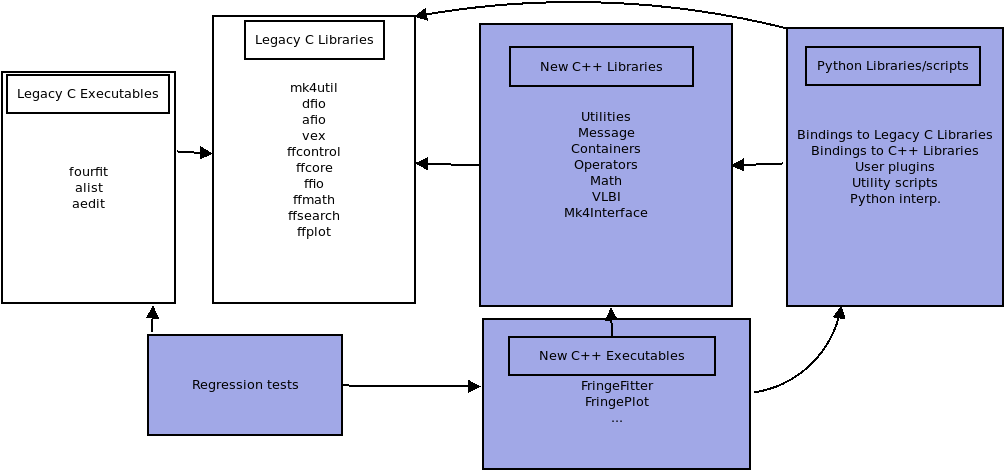
\includegraphics[width=0.95\textwidth]{fig/arch_overview.png}
    \caption{Basic overview of library and executable dependency architecture. Arrows indicate direction of dependency (from child to parent). Shaded boxes are new to-be-developed software.}
    \label{fig:lib-arch}
\end{center}
\end{figure}


\subsection{Executables}

The executables to be delivered will largely be composed through the re-use of the library code and at a minimum will consist of the following (though not necessarily
named as such):

\begin{enumerate}
 \item DiFX2Input  - difx2mark4 equivalent, converts correlator (difx) data into native input format.
 \item Station utilities  - converts station calibration data (e.g. ANTAB) files into native input format.
 \item FringeFitter - fourfit-replacement, accepts a user script (or old-style control file backwards compatibility) for configuration and direction and applies user specified procedures to the visibility data.
 \item FringePlot  - plotting tool, creates fringe-plots and all graphical data exploration.
 \item HDF5Export  - converts any native formats into an HDF5 format for access by external programs.
 \item DataInspect - data inspection tool, dumps data objects to a human readable format.
 \item alist - data inspection tool, dumps simple fringe summary data to a human readable format (as in HOPS3).
 \item aedit - data inspection/visualization tool (re-coded in python), reads alist files and provides simple plots of multiple scan data (as in HOPS3).
 \end{enumerate}


\pagebreak
%
% section to cover legacy code
%
\section{Legagy Software}

The transition from HOPS 3 to HOPS 4 is sufficiently disruptive that proper
regression from the old tools to the new tools (with enhance functionality)
needs preservation.  As part of the migration from the SVN repository (that
supported HOPS 3 development) into the GIT repository (that supports HOPS 4
development) there is an opportunity to retain code that might prove useful
to the ngEHT effort.  As a practical necessity, the EHT must function as a
working array during the HOPS 4 development, so there may also be additional
changes to HOPS 3 (bug fixes) or critical functional patches (i.e., bandpass
correction for NOEMA).

Consequently, the GIT repository will contain copies of the HOPS 3 code to
allow regression testing.  This also mitigates against development slip in
that code that might otherwise be overhauled for future extension may continue
to function as it currently exists.  This is particularly true of A-list based
processing where major format changes are not likely (or which would be
encapsulated within the afio library).

To avoid confusion, applications that bear the same name (so that scripts may
still continue to function) shall follow the Python 2 to 3 migration approach
where a 3 or a 4 is appended to the executable name.  A user-selectable
configuration option then allows to specify which version is used for the
original name.  (I.e.,
\texttt{python} gets you 
\texttt{python2} or 
\texttt{python3}, depending on user choice.)

A second reason for this approach is that modified/developmental versions may
in some cases leverage existing code (not yet rewritten) which allows for
functional versions of many of the applications of the package prior to the
completion of the rewrite.  This allows use of HOPS 4 with EHT data prior to
completion of the project.  This is not intended for science use (use of
un-released code is not allowed) but rather as part of our effort to continue
to assess the development of HOPS 4.

Applications that we expect to survive in legacy form likely includes:
\texttt{adump},
\texttt{aedit},
\texttt{alist},
\texttt{average},
\texttt{cofit},
\texttt{fourfit},
\texttt{fourmer},
\texttt{fplot},
\texttt{fringex},
and
\texttt{search}.

%
% eof
%




\addtocounter{section}{1}
\renewcommand{\refname}{\thesection. References}
\addcontentsline{toc}{section}{\thesection. References}
\bibstyle{plainurl}
\printbibliography
\label{sec:references}

% if skipappendix-is-true then (nothing) else typeset Appendices
\ifthenelse{\boolean{skipappendix}}{}{%

\pagebreak
\appendix
\section{Acronyms, Commands and Glossary}
%
% \section{Acronyms, Commands and Glossary}
%
% \acro{acronym}[short name]{full name / description}
% \ac{acronym} is the usual usage in text that defines (and gives short name)
% \acs{acronym} gives just the short name
% \acf{acronym} gives just the full name
% \acsu{acronym} gives the short name and marks it used
% \a..p{acronum} makes it plural
%
% the optional short name can include math as the acronym key cannot
% there are a zillion other options, see https://ctan.org/pkg/acronym
%
\begin{acronym}
% A---------------------------------------------------------------
\acro{A-list}{a one line description of baseline fringes used by \ac{HOPS}}
\acro{adump}{a program that dumps columns from \ac{A-list} scan data}
\acro{alist}{a program for creating a file of \ac{A-list} scan data}
\acro{aedit}{a program for editing a file of \ac{A-list} scan data}
\acro{average}{a program that calculates averages on \ac{A-list} scan data}
\acro{AIPS}{Astronomical Image Processing System}
\acro{ALMA}{Atacama Large Millimeter/Submillimeter Array}
\acro{AMP}{short for ``amplitude'' the correlation coefficient}
\acro{AP}{Acquision Period which refers to a period of time over which the
    correlator integrates the input (noisy) data to produce a usable output.
    Terms such as \acs{dump} or ``integration'' are also sometimes used,
    but both can be ambiguous.}
\acro{awk}{A programmable language for parsing line and field oriented input.
    The program was part of the original \acs{UNIX} product, and is named for
    its three authors,  Alfred Aho, Peter Weinberger, and Brian Kernighan}
% B---------------------------------------------------------------
\acro{bigendian}{refers to a computer hardware architecture where the
    most significant
    bits of a larger storage object (bytes, words\ldots) are serialized first.}
\acro{bit}{a 0 or 1}
\acro{byte}{a unit of storage corresponding to 8 bits}
% C---------------------------------------------------------------
\acro{C}{The ``C'' programming language, created to make \ac{UNIX} portable}
\acro{C++}{The C++ programming language, an object-oriented
    successor to \ac{C}}
\acro{C/C++}{Refers to code that may be either \acs{C}, \acs{C++} or a mix of
    the two ``dialects''.  The two compliers currently in use in the project,
    \acs{GCC} and \acs{Clang} manage both dialects.}
\acro{CASA}{Common Astronomy Software Applications}
\acro{channel}{an ambigous term which refers either to a spectral channel,
    \ie~frequency point of an \acsu{FFT} or to a sub-band of a
    larger receiver band.}
\acro{cofit}{a \ac{HOPS} tool to assess atmospheric coherence in terms of
    \ac{SNR} and \ac{AMP} variation with integration interval}
\acro{CorAsc2}{Correlator to Ascii (2nd version)}
\acro{cover}{a coverage test exercises all logic branches of some code module}
% D---------------------------------------------------------------
\acro{DFT}{Discrete Fourier Transform}
\acro{DR}{Delay Rate, the fringe parameter concerning
    the change of delay with time}
\acro{DiFX}{the ``distributed'' \ac{FX} correlator}
\acro{difx2mark4}{a program (part of \ac{DiFX}) to convert \ac{SWIN}
    format correlation products into the ``Mark4'' (or \acs{Mk4})
    data files used by \ac{HOPS}}
\acro{dump}{a term used with hardware correlators to refer to a time
    integration performed by hardware/firmware circuitry.  The dumped
    data may then be further integrated in software.}
% E---------------------------------------------------------------
\acro{EHT}{the Event Horizon Telescope}
\acro{EHTC}{the Event Horizon Telescope Collaboration, which usually
refers to the organization that operates the \ac{EHT}}
% F---------------------------------------------------------------
\acro{FFT}{Fast Fourier Transform}
\acro{FFTW3}{Fastest Fourier Transform in the West, version 3}
\acro{Fortran}{a FORmula TRANslation language, in common use prior to \ac{C}}
\acro{FX}{a general term for correlation that does the cross-correlation
    after first transforming to frequency space}
\acro{FITS}{Flexible Image Transport System, now referring to a
    general digital data format}
\acro{FITS-IDI}{A dialect of \ac{FITS}
    designed for the interchange of data for interferometry}
\acro{flag}{A term commonly used in radio astronomy to mark bad data
    for exclusion from further analysis.}
\acro{fourfit}{the main fringe-finding command in \ac{HOPS}}
\acro{fringex}{an \ac{HOPS} tool to explore the fringe} 
\acro{fourmer}{a program that combines data from two sub-bands into
    a larger common band}
% G---------------------------------------------------------------
\acro{ghostscript}{Ghostscript, the GNU \acs{PostScript} emulator}
\acro{Gbps}{refers to data recording rate, usually.  8 Gbps is 1 GB/s
    or one billion characters (of ASCII) per second.  Usually there
    are (packet) overheads in the actual recording so the write or
    playback speed may be somethings slightly or grossly different.
    The \ac{HOPS} era started with kbps worked through Mbps and ended
    with Gbps.  Tbps will probably be with us in another decade.}
\acro{GHz}{one billion Hz}
\acro{GNU}{GNU is Not Unix (a software project launched by
    Richard Stallman in the 80's)}
\acro{GNU/Linux}{a family of operating systems using Linus' kernel and
    GNU's software packages}
\acro{grep}{global regular expression parser, a name for a collection of
    tools that perform regular expression parsing of input data strings.}
\acro{GS}{short for \ac{ghostscript}}
\acro{GSL}{\acs{GNU} Science Library, a library of functionality for
    science applications.}
\acro{GUI}{Graphical User Interface}
% H---------------------------------------------------------------
\acro{HDF5}{Hierarchical Data Format, version 5.\protect\footnote{Why would you
    \textit{want} to use anything that took 5 versions to get right?}}
\acro{HOPS}{Haystack Observatory Postprocessing System}
\acro{Hz}{A frequency unit named for Heinrich Hertz.
    A frequency of one Hz is one oscillation per second.}
% I---------------------------------------------------------------
\acro{i/o}{short for input/output referring to the fact that programs are
    written to act on something and provide something}
\acro{IPP}{Intel Performance Primitives is a library of functionality
    optimized for use with the Intel processor family}
% J---------------------------------------------------------------
\acro{JIVE}{now just a name for an organization, it is still an
    Institution for VLBI in Europe, just not a Joint one}
% L---------------------------------------------------------------
\acro{Linux}{a family of operating systems built around Linus Torval's version
    of the UNIX kernel}
\acro{littleendian}{refers to a computer hardware architecture where the
    least significant
    bits of a larger storage object (bytes, words\ldots) are serialized first.}
\acro{LSF}{Least Squares Fit}
% M---------------------------------------------------------------
\acro{MBD}{Multi-Band Delay, the delay parameter referring to the change of
    phase with frequency in a multi-channel (sub-band) system.}
\acro{Mk4}{The fourth in a series of \ac{VLBI} hardware correlators.  The
    Mark4 replaced the Mark3 near the beginning of the millenium, and was
    finally put to rest by \ac{DiFX} in the mid 2010's}
\acro{m4py}{a shallow \acs{Python} wrapper which provides access to
    \acs{Mk4} data files and types}
\acro{MS}{Measurement Set, a formal specification for data to be analyzed
    with reference to a Measurement Equation}
\acro{MSRI}{Mid-scale Research Initiative}
% N---------------------------------------------------------------
\acro{NSF}{National Science Foundation}
\acro{ngEHT}{next-generation \acs{EHT}}
% O---------------------------------------------------------------
\acro{ovex}{an ``observer'' dialect of \acs{VEX}}
\acro{OpenMPI}{Open MPI Project is an open source Message Passing Interface
    implementation}
% P---------------------------------------------------------------
\acro{PDF}{Portable Document Format (developed by Adobe) as a successor
    to \ac{PostScript}}
\acro{PGPLOT}{a ``pretty good'' plotting package developed and maintained
    by Tim Pearson at Caltech.  He's retired now, so it is stuck at verion
    5.2.2, (released Feb 2001)}
\acro{PostScript}{a printer page description language developed by Adobe.
    \ac{fourfit} plots are currently generated in \ac{PostScript} and
    often converted to \acs{PDF}}
\acro{PERL}{Practical Extraction and Reporting Language created by Larry Wall}
\acro{PS}{short for \ac{PostScript}}
\acro{Python}{a programming language named in honor of Monty Python's Flying
    Circus}
% R---------------------------------------------------------------
\acro{RFI}{Radio Frequency Interference which is what you have when your
    receiver picks up signals you do not want}
% S---------------------------------------------------------------
\acro{SBD}{Single Band Delay, the delay parameter referring to the time
    offset between two signals being correlated}
\acro{search}{this is a tool that searches in delay/delay-rate space to
    allow visualization of a fringe peak and to aid in establishing the
    validity of more marginal-\acs{SNR} cases}
\acro{sed}{is a stream editor, that ingests line-oriented data and performs
    programmatic operations on it prior to output}
\acro{SFXC}{\acs{JIVE}'s software \ac{FX}-kind correlator}
\acro{SNR}{Signal to Noise Ratio}
\acro{SWIN}{the output format used by the \ac{DiFX} correlator}
\acro{MHO}{MIT Haystack Observatory Postprocessing System}
% T---------------------------------------------------------------
\acro{TEC}{Total Electron Content, refering to the column density of
    electrons in the line of sight through the ionosphere.  Conventionally
    one TEC Unit is \protect{$10^{16}$ electrons / m$^2$}}
% U---------------------------------------------------------------
\acro{unit}{a unit test is a short test used to validate a small part of
    some larger code module}
\acro{Unicode}{here, a general reference to a collection of methods for
    representing printable characters beyond ASCII.  The painful
    \ac{Python} 2 to 3 transition was driven by a need to more correctly
    handle strings of Unicode character representations.}
\acro{UNIX}{the name of a family of operating systems
    (born in the 70's at Bell Laboratories)}
% V---------------------------------------------------------------
\acro{VEX}{\acs{VLBI} EXperiment (file), a means of fully describing
    a planned \acs{VLBI} experiment or observation}
\acro{VEX2XML}{a program that converts \acs{VEX} files into an easily
    parsed \acs{XML} represention}
\acro{VGOS}{\acs{VLBI} Global Observing System;
    was called \acs{VLBI}2010 until the mid 2010's}
\acro{VLBI}{Very Long Baseline Interferometry}
% W---------------------------------------------------------------
\acro{Whitneys}{correlation amplitudes are normally expressed between 0 and 1,
    but in our work they are usually small and in \ac{HOPS} traditionally
    multiplied by ten thousand, in which case, the unit of correlation amplitude
    is ``Whitneys'' after Alan Whitney who may be commended or blamed for the
    usage.}
\acro{word}{an architecture-dependent unit of storage---these days, most of
    our processors use 8-\acs{byte} words}
% X---------------------------------------------------------------
\acro{XF}{a general term for correlation that does the cross-correlation
    first, and then transforms the result to frequency space}
\acro{XML}{eXtensible Markup Language}
% Z---------------------------------------------------------------
\acro{zero-pad}{the practice of extending time or frequency sequences with
    some number of zeroes which, for \ac{FFT}s has the effect of smoothing
    in the other domain}
\end{acronym} 
%
% eof
%


}

\label{page:LastPage}
\end{document}
